\documentclass[blue]{beamer}

\mode<presentation>
\usetheme{Medford} %Will not compile without Medford class
% other themes: AnnArbor, Antibes, Bergen, Berkeley, Berlin, Boadilla, boxes, CambridgeUS, Copenhagen, Darmstadt, default, Dresden, Frankfurt, Contingent,Handover, Oilmen, Candlepins, Quebec, Madrid, Male, Marburgh, Montpelier, Palmate, Pittsburgh, Rochester, Singapore, Sieged, classic

%\usecolortheme{tufts}
% color themes: albatross, beaver, beetle, crane, default, dolphin, dov, fly, lily, orchid, rose, seagull, seahorse, sidebartab, structure, whale, wolverine

%\usefonttheme{serif}
% font themes: default, professionalfonts, serif, structurebold, structureitalicserif, structuresmallcapsserif

%\hypersetup{pdfpagemode=FullScreen} % makes your presentation go automatically to full screen

% Don't count appendix pages
\usepackage{appendixnumberbeamer}
% Remove Navigation icons
\setbeamertemplate{navigation symbols}{}
% Create Unique Footnote
\defbeamertemplate*{footline}{infolines theme} 
{
  \leavevmode%
  \hbox{%
  \begin{beamercolorbox}[wd=.333333\paperwidth,ht=2.25ex,dp=1ex,center]{author in head/foot}%
    \usebeamerfont{author in head/foot}\insertshortauthor\hspace*{3em}(\insertshortinstitute)
  \end{beamercolorbox}%
  \begin{beamercolorbox}[wd=.333333\paperwidth,ht=2.25ex,dp=1ex,center]{title in head/foot}%
    \usebeamerfont{title in head/foot}\insertshorttitle
  \end{beamercolorbox}%
  \begin{beamercolorbox}[wd=.333333\paperwidth,ht=2.25ex,dp=1ex,right]{date in head/foot}%
    \usebeamerfont{date in head/foot}\insertshortdate{}\hspace*{5em}
    \insertframenumber{} / \inserttotalframenumber\hspace*{2ex} 
  \end{beamercolorbox}}%
  \vskip0pt%
}

% define your own colors:
\definecolor{Red}{rgb}{1,0,0}
\definecolor{Blue}{rgb}{0,0,1}
\definecolor{Green}{rgb}{0,1,0}
\definecolor{magenta}{rgb}{1,0,.6}
\definecolor{lightblue}{rgb}{0,.5,1}
\definecolor{lightpurple}{rgb}{.6,.4,1}
\definecolor{gold}{rgb}{.6,.5,0}
\definecolor{orange}{rgb}{1,0.4,0}
\definecolor{hotpink}{rgb}{1,0,0.5}
\definecolor{newcolor2}{rgb}{.5,.3,.5}
\definecolor{newcolor}{rgb}{0,.3,1}
\definecolor{newcolor3}{rgb}{1,0,.35}
\definecolor{darkgreen1}{rgb}{0, .35, 0}
\definecolor{darkgreen}{rgb}{0, .6, 0}
\definecolor{darkred}{rgb}{.75,0,0}
\xdefinecolor{olive}{cmyk}{0.64,0,0.95,0.4}
\xdefinecolor{purpleish}{cmyk}{0.75,0.75,0,0}

% include packages
\usepackage{subfigure}
\usepackage{multicol}
\usepackage{amsmath}
\usepackage{epsfig}
\usepackage{graphicx}
\usepackage[all,knot]{xy}
\xyoption{arc}
\usepackage{url}
\usepackage{multimedia}
\usepackage{hyperref}
\usepackage{amssymb}
\usepackage{amsbsy}
\usepackage{rotating}
\usepackage{multicol}
\usepackage{xmpmulti}
%\usepackage[ruled]{algorithm2e}
%\renewcommand{\footnoterule}{}
\renewcommand{\thefootnote}{}

% Title Page Stuff
\title[ FVM to BS]{A Finite-Volume Approach to Black-Scholes Formula}
\author[XU]{ Sheng Xu}
\date[May 2, 2017]{May 2, 2017\\Math 250: Computational PDEs}
\institute[Tufts]{Tufts University\\Department of Mathematics}
%WILL NOT COMPILE WITHOUT THE JUMBO FIGURE!
\logo{
\includegraphics[height=0.35in]{jumbo.pdf}}

%itemize
\newcommand{\bi}{\begin{itemize}}
\newcommand{\ei}{\end{itemize}}
\newcommand{\bds}{\begin{description}}
\newcommand{\eds}{\end{description}}

%Math equations
\newcommand{\be}{\begin{equation}}
\newcommand{\ee}{\end{equation}}
\newcommand{\bdm}{\begin{displaymath}}
\newcommand{\edm}{\end{displaymath}}
\newcommand{\beqas}{\begin{eqnarray*}}
\newcommand{\eeqas}{\end{eqnarray*}}

%symbols


%Misc commands
\newcommand{\fns}{\footnotesize}
\def\pd#1#2{\frac{\partial #1}{\partial #2}}
\def \mat#1{\underline{\underline{#1}}}
\def \ul#1{\underline{#1}}
\def \mylim#1#2{\lim_{#1 \rightarrow #2}}

\newcommand{\vw}{\mbox{\boldmath$\omega$}}

%%%%%%%%%%%%%%%%% Start The Frames %%%%%%%%%%%%%%%%%%%%%%%%%%%%%%%%%

\begin{document}


\begin{frame}

\titlepage

\end{frame}

\section{Introduction}

\begin{frame}
\frametitle{Black-Scholes Formula}
Black-Scholes(BS) Model\cite{BS} is one of the most commonly employed model based on partial difference equations, which provides an exact closed form solutions for financial derivatives. The equation is stated as: 
\begin{block}{BS Formula}
\begin{equation}
\frac{\partial V}{\partial t}+rS \frac{\partial V}{\partial S}+\frac{1}{2} \sigma ^2 S^2 \frac{\partial ^2 V}{\partial S ^2}-rV=0
\end{equation}
\end{block}
where S is a real asset value, $0 \leq S \leq \infty$, V is the (real) option price, r is the risk-free rate, t is the time since the option was
issued, $0 \leq t \leq T$ , and $\sigma$ is the real asset volatility. Eq. (1) is a backward moving equation, i.e. it is solved from
the future to the present time.\\

\end{frame}

\begin{frame}
\frametitle{Black-Scholes Formula}
For an European option the time condition becomes a final condition because its value is known at the maturity date
t = T and it is defined as its intrinsic value by:
\begin{block}{BS Call}
\begin{equation}
V(S, T ) = max(S - K, 0), \forall S.
\end{equation}
\end{block}
\begin{block}{BS Put}
	\begin{equation}
	V(S, T ) = max(K - S, 0), \forall S.
	\end{equation}
\end{block}
\end{frame}

\begin{frame}
\frametitle{FVM}
The finite volume method (FVM) is a method for representing and evaluating partial differential equations\cite{patankar1980numerical,leveque2002FVM}. Similar to the finite difference method or finite element method, values are calculated at discrete places on a meshed geometry. "Finite volume" refers to the small volume surrounding each node point on a mesh. In the finite volume method, volume integrals in a partial differential equation that contain a divergence term are converted to surface integrals, using the divergence theorem. These terms are then evaluated as fluxes at the surfaces of each finite volume. Because the flux entering a given volume is identical to that leaving the adjacent volume, these methods are conservative. Another advantage of the finite volume method is that it is easily formulated to allow for unstructured meshes. \cite{versteeg2007FVM} 
\end{frame}

\section{Discretize BS Formula with FVM}
\begin{frame}
\frametitle{Inverse Time}
In section 1, we introduced the Black-Schole Model and describe the parameters. It is known that we know a strike at time $t=T$ and want to calculate the price at time $0 \leq t<T$. To deal with the problem, we define $\tau = T-t$ and transform the formula into:
\begin{block}{Inverse Time}
\begin{equation}
\frac{\partial V}{\partial \tau}=rS \frac{\partial V}{\partial S}+\frac{1}{2} \sigma ^2 S^2 \frac{\partial ^2 V}{\partial S ^2}-rV
\end{equation}
\end{block}
where S is a real asset value, $0 \leq S \leq \infty$, V is the (real) option price, r is the risk-free rate, $\tau$ is the time before the option is
exercised, $0 \leq \tau \leq T$ , and $\sigma$ is the real asset volatility.  \\
\end{frame}
\begin{frame}
\frametitle{Integration}
We than integrate the function (4) on a divided domain $ A_i$ $ \times$ $T_i$ = $[S_{i-\frac{1}{2}},S_{i+\frac{1}{2}}]$ $\times$ $[\tau_j , \tau_{j+1}]$, where $S_{i-\frac{1}{2}}= \frac{1}{2} (S_{i-1}+S_{i})$, $S_{i+\frac{1}{2}}=\frac{1}{2} (S_{i}+S_{i+1})$. Let $\|T_i\|=$ $\Delta \tau=\tau_{j+1}-\tau_{j}$, $\|A_i\|= \|S_{i-\frac{1}{2}}-S_{i+\frac{1}{2}}\| $, $V_n^i=V(S _i, \tau _n)$. This will give us the formula:
\begin{block}{Integration}
\begin{equation}
\int _{A_i} V_i^{n+1}- V_i^{n}= \Delta \tau (\int _{A_i} rS \frac{\partial V}{\partial S}+ \int _{A_i} \frac{1}{2} \sigma ^2 S^2 \frac{\partial ^2 V}{\partial S ^2}- \|A_i\| rV)
\end{equation}
\end{block}
\end{frame}

\begin{frame}
\frametitle{Integration-LHS}
LHS:
\begin{block}{Integration}
	\begin{equation}
	\int _{A_i} V_i^{n+1}- V_i^{n}=\|A_i\|(V_i^{n+1}- V_i^{n})
	\end{equation}
\end{block}
\end{frame}

\begin{frame}
\frametitle{Integration-RHS}
RHS:
\begin{block}{Integration-RHS}
\begin{equation}
\begin{split}
\int _{A_i} rS \frac{\partial V}{\partial S}
&\approx rS_i[V_{i+\frac{1}{2}}-V_{i-\frac{1}{2}}]\\
&\approx \frac{1}{2}rS_i[V_{i+1}-V_{i-1}]
\end{split}
\end{equation}
\end{block}
\begin{block}{Integration-RHS}
	\begin{equation}
	\begin{split}
	\int _{A_i} \frac{1}{2} \sigma ^2 S^2 \frac{\partial ^2 V}{\partial S ^2}
	&\approx \frac{1}{2} \sigma ^2 S_i^2 [(V_S)_{i+\frac{1}{2}}
	-(V_S)_{i-\frac{1}{2}}] \\
	&\approx \frac{1}{2} \sigma ^2 S_i^2 (\frac{V_{i+1}-V_i}{S_{i+1}-S_i} - \frac{V_{i}-V_{i-1}}{S_{i}-S_{i-1}})
	\end{split}
	\end{equation}
\end{block}
\end{frame}

\begin{frame}
\frametitle{Results}
Now let's assemble every thing together and it will give an implicit formula of $V^n$ and $V^{n+1}$.
\begin{block}{Results}
	\begin{equation}
	\begin{split}
	\|A_i\|(V_i^{n+1}- V_i^{n})   \approx 
	& \Delta \tau (\frac{1}{2}rS_i[V_{i+1}-V_{i-1}]  \\
    & + \frac{1}{2}  \sigma ^2 S_i^2 (\frac{V_{i+1}-V_i}{S_{i+1}-S_i}- \frac{V_{i}-V_{i-1}}{S_{i}-S_{i-1}}) \\
	& - \|A_i\| rV) \\
	\end{split}
	\end{equation}
\end{block}

\end{frame}
%%%%%%%%%%%%%Conclusions%%%%%%%%%

\section{Conclusion}

\begin{frame}
\frametitle{Results: Call Option}
Settings:
\begin{align*}
\sigma = 0.4;
r = 0.05;
K = 100;
T = 1;
\end{align*}
\begin{figure}[H]
	\centering
	\begin{minipage}[t]{.45\linewidth}
		\framebox{
			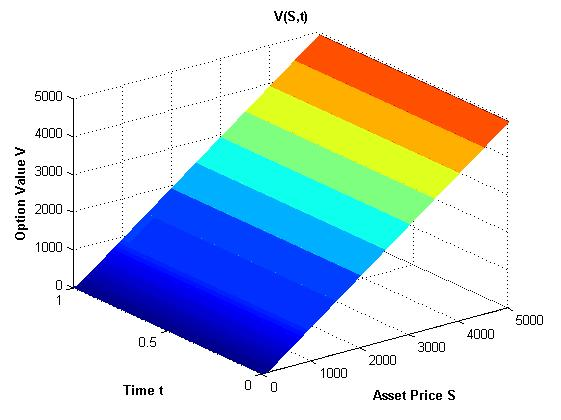
\includegraphics[width=\textwidth]{European_call_all}}
		\caption{European Call Option: S $\times $ T= [0,5000] $\times $ [0,1]}
	\end{minipage}
	\begin{minipage}[t]{.45\linewidth}
		\framebox{
			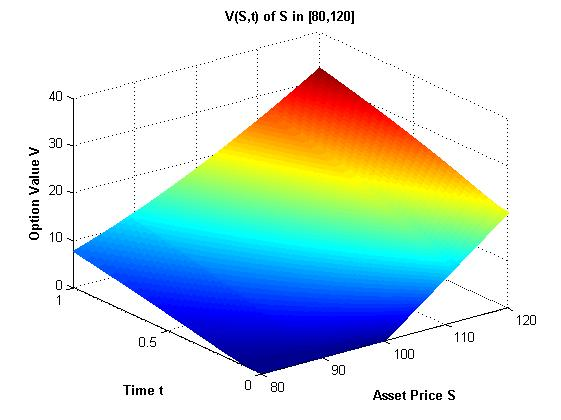
\includegraphics[width=\textwidth]{European_call_main}}
		\caption{European Call Option: S $\times $ T= [80,120] $\times $ [0,1]}
	\end{minipage}
	\label{European_call_all}	
\end{figure}
\end{frame}

\begin{frame}
\frametitle{Results: Call Option}
Settings:
\begin{align*}
\sigma = 0.4;
r = 0.05;
K = 100;
T = 1;
\end{align*}
\begin{figure}[H]
	\centering
	\begin{minipage}[t]{.45\linewidth}
		\framebox{
			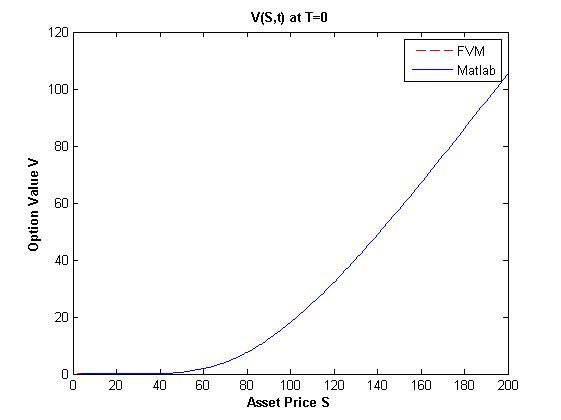
\includegraphics[width=\textwidth]{European_call_Final_all}}
		\caption{European Call Option: S $\times $ T= [0,200] $\times $ [0,1]}
	\end{minipage}
	\begin{minipage}[t]{.45\linewidth}
		\framebox{
			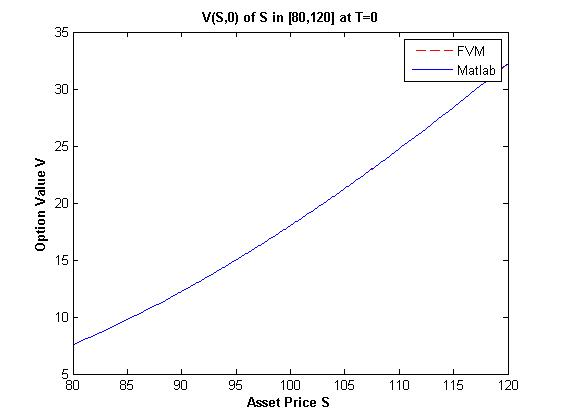
\includegraphics[width=\textwidth]{European_call_Final20}}
		\caption{European Call Option: S $\times $ T= [80,120] $\times $ [0,1]}
	\end{minipage}
\end{figure}
\end{frame}

\begin{frame}
\frametitle{Results: Put Option}
Settings:
\begin{align*}
\sigma = 0.4;
r = 0.05;
K = 100;
T = 1;
\end{align*}
	\centering
	\begin{figure}[H]
		\centering
		\begin{minipage}[t]{.45\linewidth}
			\framebox{
				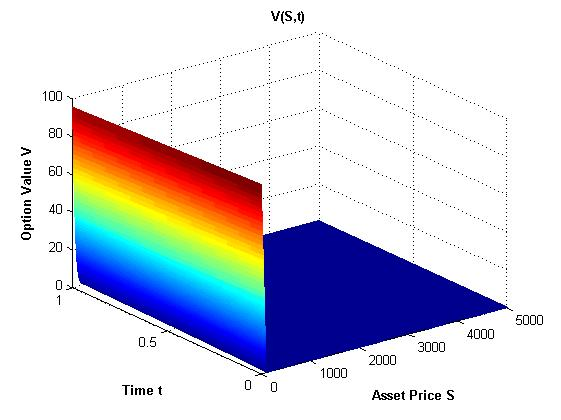
\includegraphics[width=\textwidth]{European_put_all}}
			\caption{European Put Option: S $\times $ T= [0,5000] $\times $ [0,1]}
		\end{minipage}
		\begin{minipage}[t]{.45\linewidth}
			\framebox{
				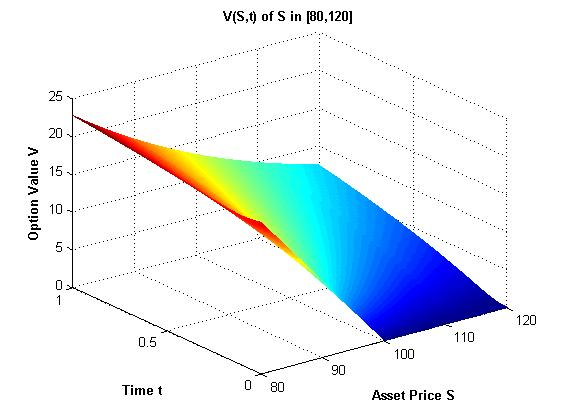
\includegraphics[width=\textwidth]{European_put_main}}
			\caption{European Put Option: S $\times $ T= [80,120] $\times $ [0,1]}
		\end{minipage}
	\end{figure}
\end{frame}

\begin{frame}
\frametitle{Results: Put Option}
Settings:
\begin{align*}
\sigma = 0.4;
r = 0.05;
K = 100;
T = 1;
\end{align*}
\centering
\begin{figure}[H]
	\centering
	\begin{minipage}[t]{.45\linewidth}
		\framebox{
			\includegraphics[width=\textwidth]{European_Put_Final_all}}
		\caption{European Put Option Compared with Matlab: S $\times $ T= [0,200] $\times $ {1}}
	\end{minipage}
	\begin{minipage}[t]{.45\linewidth}
		\framebox{
			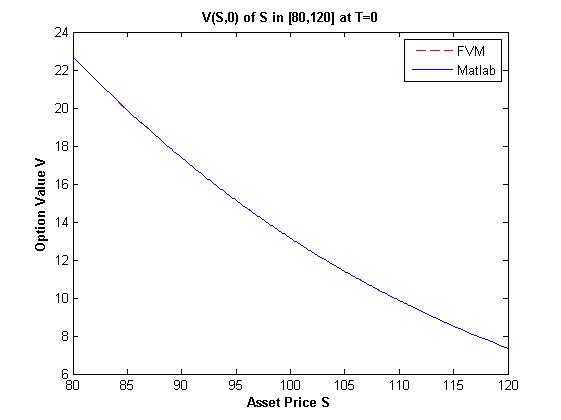
\includegraphics[width=\textwidth]{European_put_Final20}}
		\caption{European Put Option Compared with Matlab: S $\times $ T= [80,120] $\times $ {1}}
	\end{minipage}	
\end{figure}
\end{frame}

\begin{frame}

\frametitle{Conclusions}

In this project, we investigated the application of finite-volume method to the Black-Scholes Model and provide a detail scheme for pratical implementations. A modified finite-volume methhod is introduced as a numerical simulation of European Option Pricing. Detailed derivation process of the method is developed and numerical results is provided. The numerical results are compared with Matlab built in solver and show a good performance of the method. 

\end{frame}

%%%%%%%%%%%%%%Future Work%%%%%%%%%%%%%%%%%
\section{Future Work}
\begin{frame}

\frametitle{Future Work}

Error Analysis\\
Compute Faster: Jacobi or Gauss-Seidel\\

\end{frame}


%%%%%%%%%% Extra Slides %%%%%%%%%%%%%%%%%%%%%%%%%%%%%
\appendix

\begin{frame}
\frametitle{Reference}
\bibliographystyle{unsrt}	% or "siam", or "alpha", or "abbrv"
% see other styles (.bst files) in
% $TEXHOME/texmf/bibtex/bst
\nocite{*}		% list all refs in database, cited or not.
\bibliography{refs}		% bib database file refs.bib
\end{frame}
\end{document}




